\subsection{Hệ thống Shopee}
Hệ thống được nhóm lựa chọn để tham khảo là Shopee, một nền tảng thương mại điện tử đa quốc gia trực thuộc SEA Group (Singapore), hiện hoạt động mạnh tại khu vực Đông Nam Á và Đài Loan.
\\ Đường dẫn chính thức của hệ thống là: https://shopee.vn.
\\ Shopee vận hành theo mô hình sàn giao dịch điện tử trung gian, kết nối giữa người mua và người bán. Người bán có thể đăng tải sản phẩm với hình ảnh, mô tả, giá bán và tồn kho; người mua có thể tìm kiếm, thêm vào giỏ hàng, đặt hàng, thanh toán và đánh giá chất lượng sau khi nhận hàng.
\\ Quá trình vận hành bao gồm nhiều nghiệp vụ như: đăng ký và xác thực tài khoản, đăng sản phẩm, tìm kiếm, mua hàng, xử lý đơn hàng, thanh toán qua nhiều hình thức (ShopeePay, thẻ ngân hàng, COD), vận chuyển và chăm sóc khách hàng.
\\  Shopee còn tích hợp hệ thống khuyến mãi, mã giảm giá, thông báo, chat trực tiếp và quản lý tài khoản người dùng.
\subsection{Hình ảnh khảo sát}
% ảnh phần 1
\begin{figure}[H]
    \centering
    \begin{subfigure}[b]{1\textwidth}
        \centering
        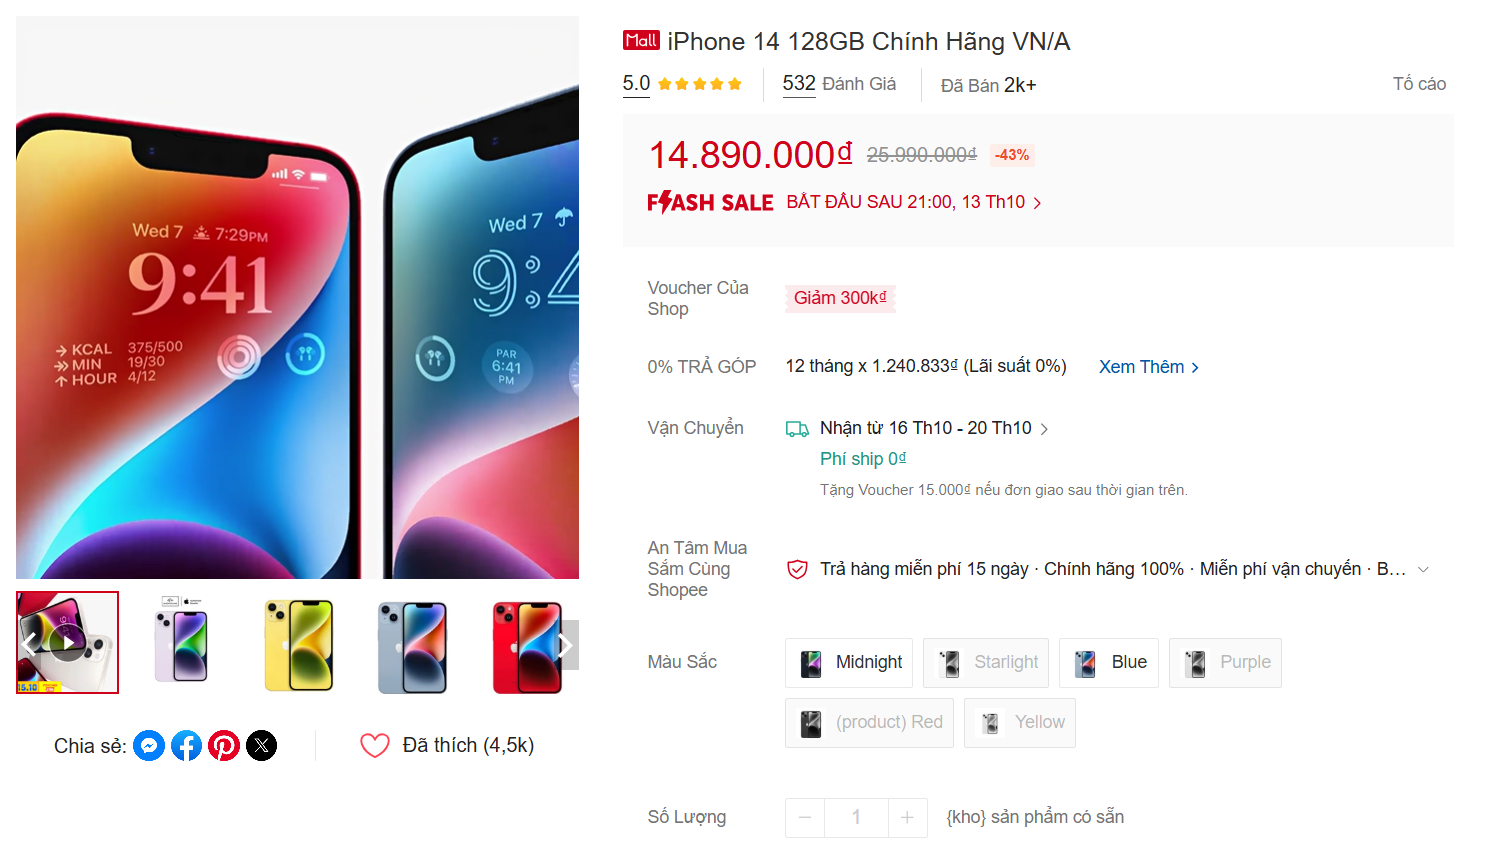
\includegraphics[width=0.9\textwidth]{Item-product_variant.png}
        \caption{Sản phẩm - loại sản phẩm}
    \end{subfigure}
    \hfill
    \begin{subfigure}[b]{1\textwidth}
        \centering
        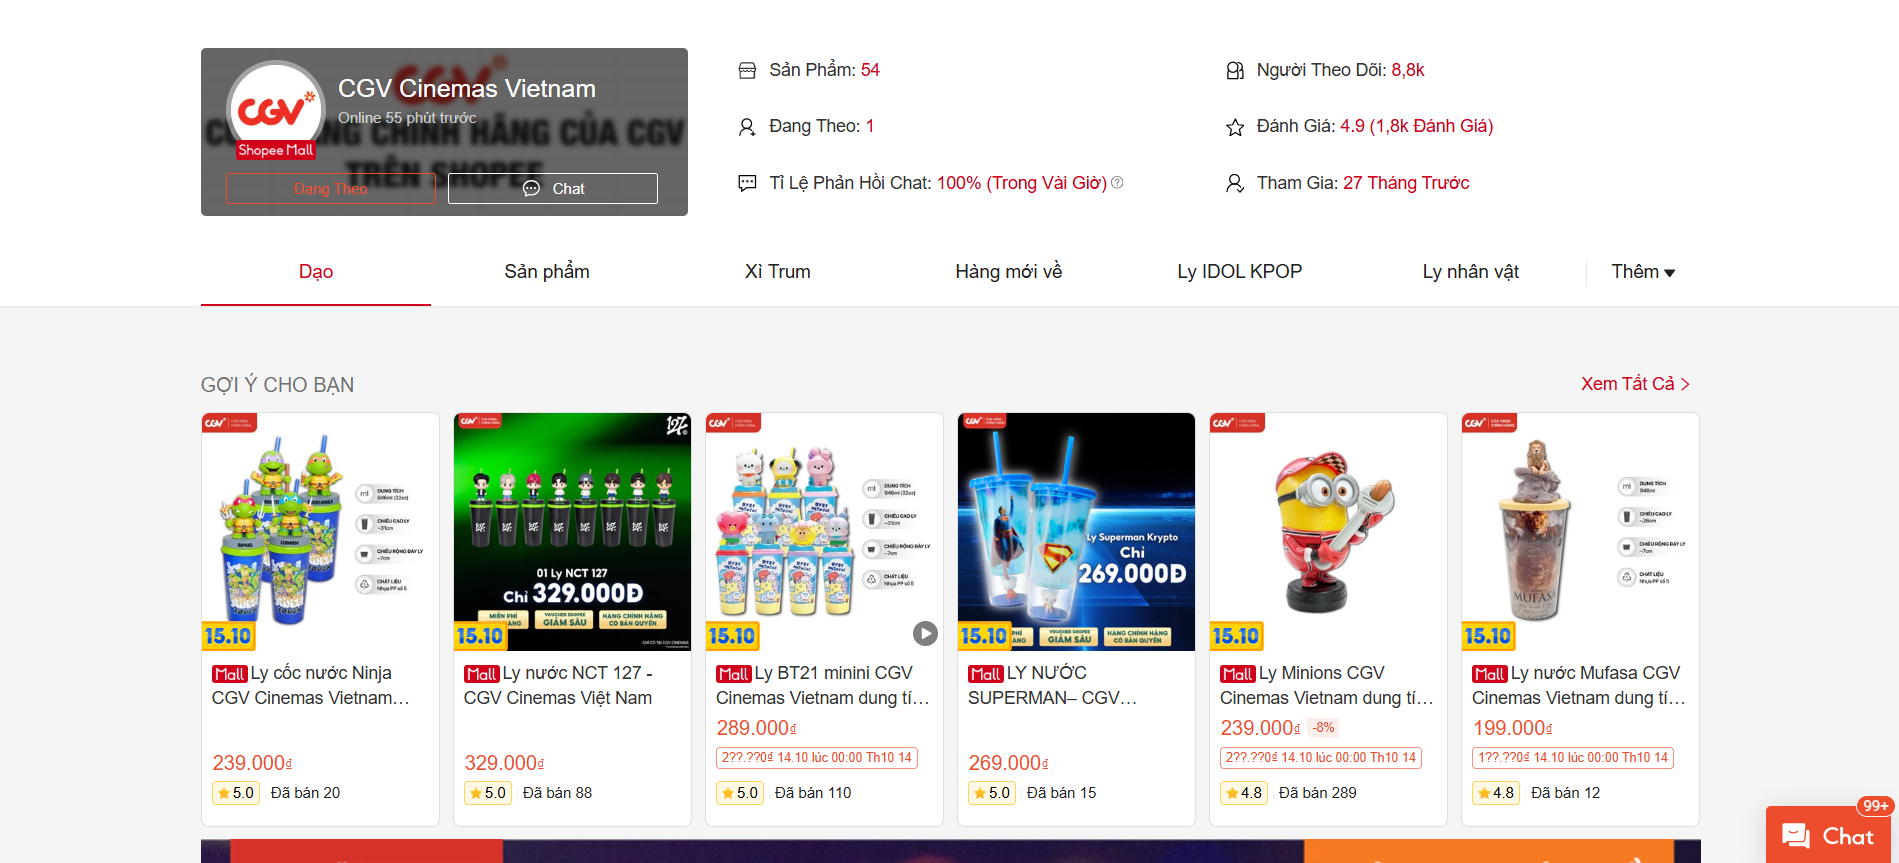
\includegraphics[width=0.9\textwidth]{Shop.png}
        \caption{Thông tin Shop}
    \end{subfigure}
    \caption{Một số hình ảnh về hệ thống Shopee}
\end{figure}
%ảnh phần 2
\begin{figure}[H]
    \centering
    \begin{subfigure}[b]{0.4\textwidth}
        \centering
        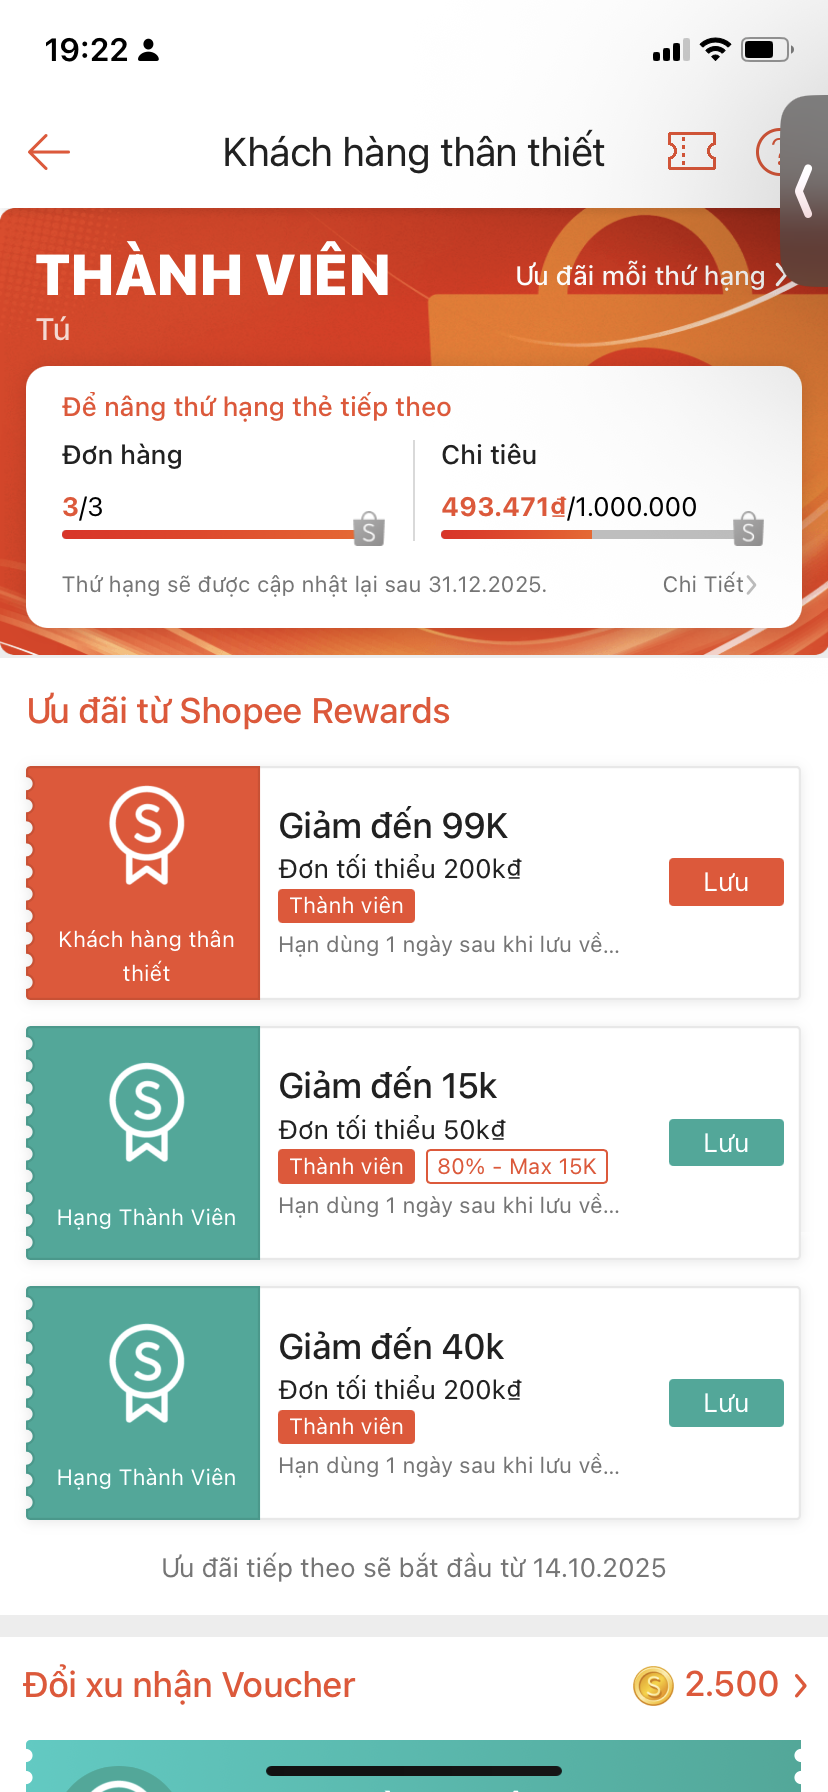
\includegraphics[width=0.6\textwidth]{Hạng_thành_viên1.PNG}
        \caption{Hạng thành viên của khách hàng}
    \end{subfigure}
    \hfill
    \begin{subfigure}[b]{0.4\textwidth}
        \centering
        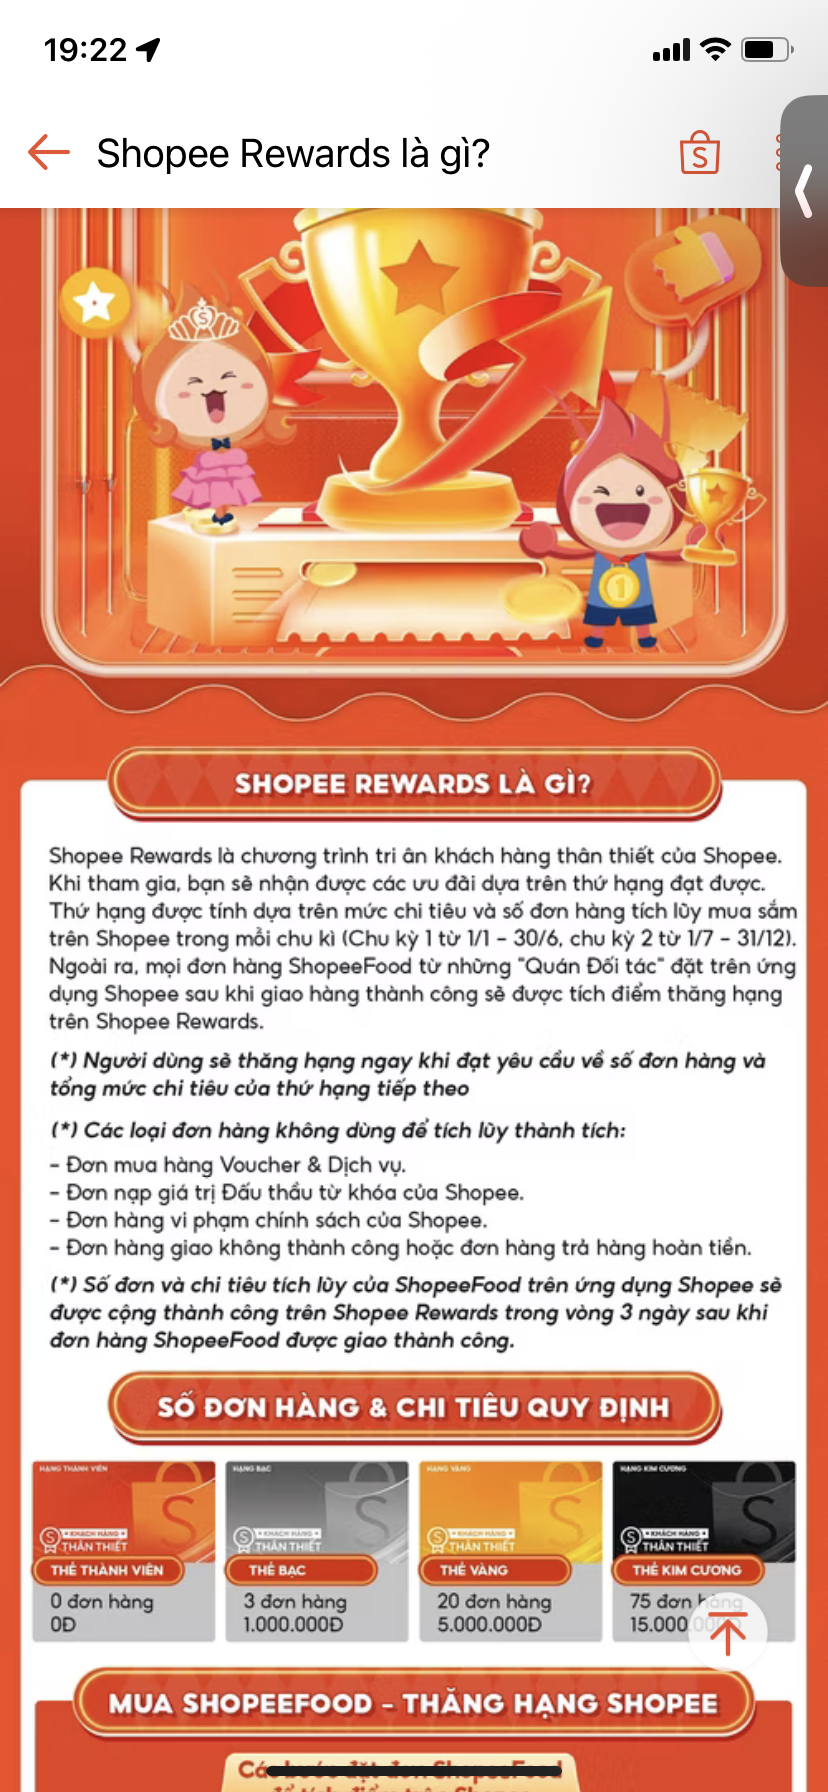
\includegraphics[width=0.6\textwidth]{Hạng_thành_viên2.PNG}
        \caption{Thông tin Hạng thành viên}
    \end{subfigure}
    \caption{Một số hình ảnh về hệ thống Shopee (tt)}
\end{figure}
%ảnh phần 3
\begin{figure}[H]
    \centering
    \begin{subfigure}[b]{0.4\textwidth}
        \centering
        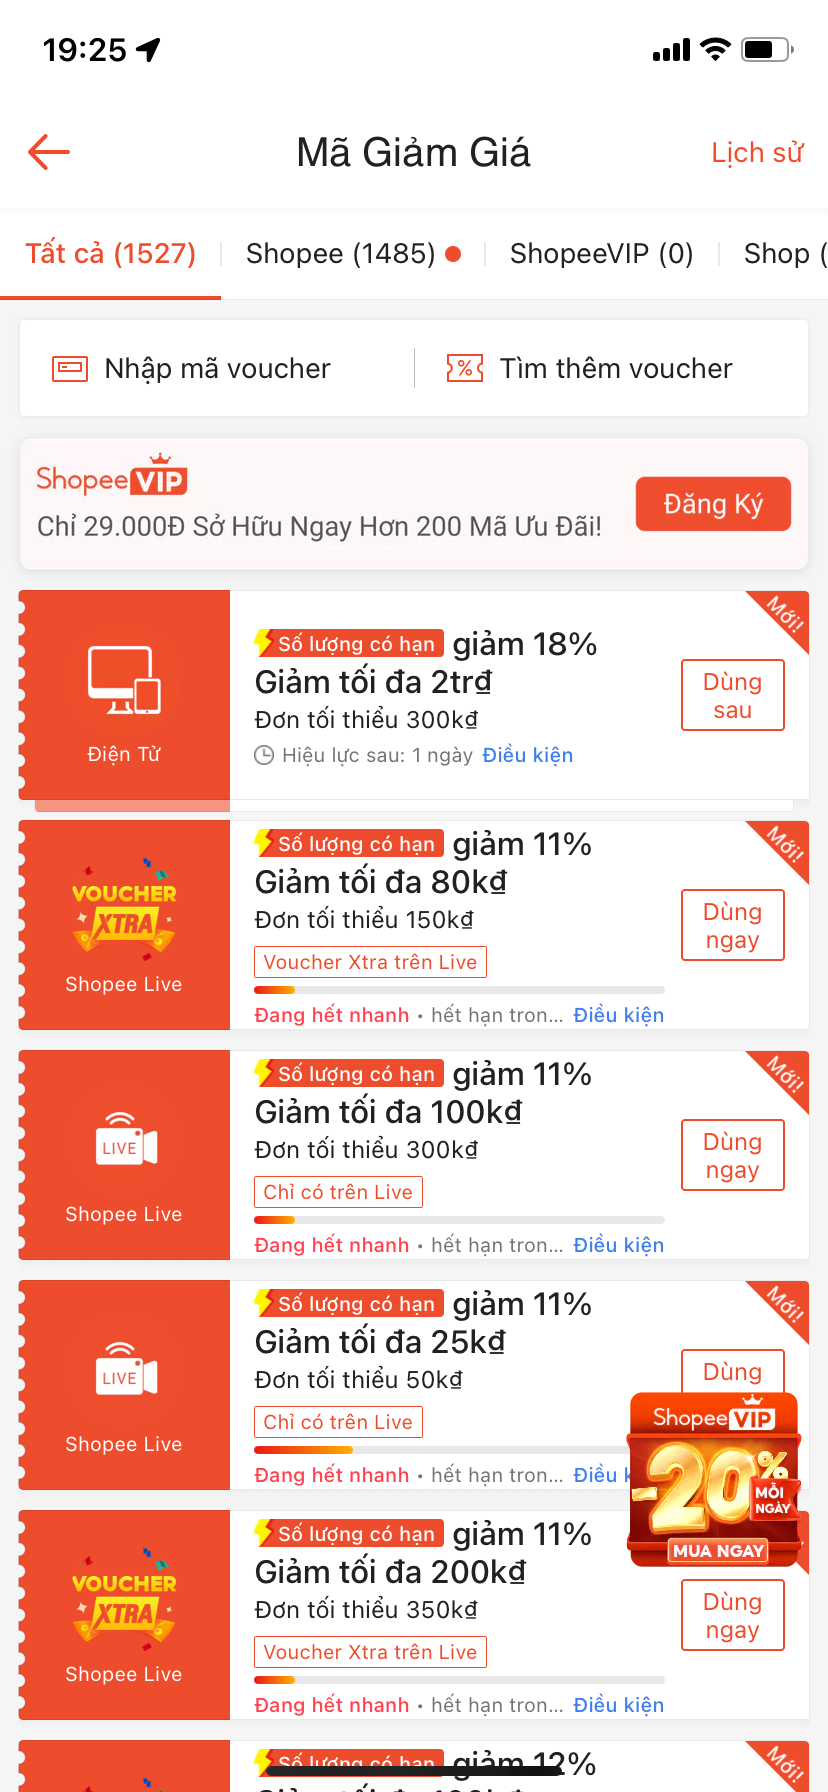
\includegraphics[width=0.6\textwidth]{Voucher.PNG}
        \caption{Voucher}
    \end{subfigure}
    \hfill
    \begin{subfigure}[b]{0.4\textwidth}
        \centering
        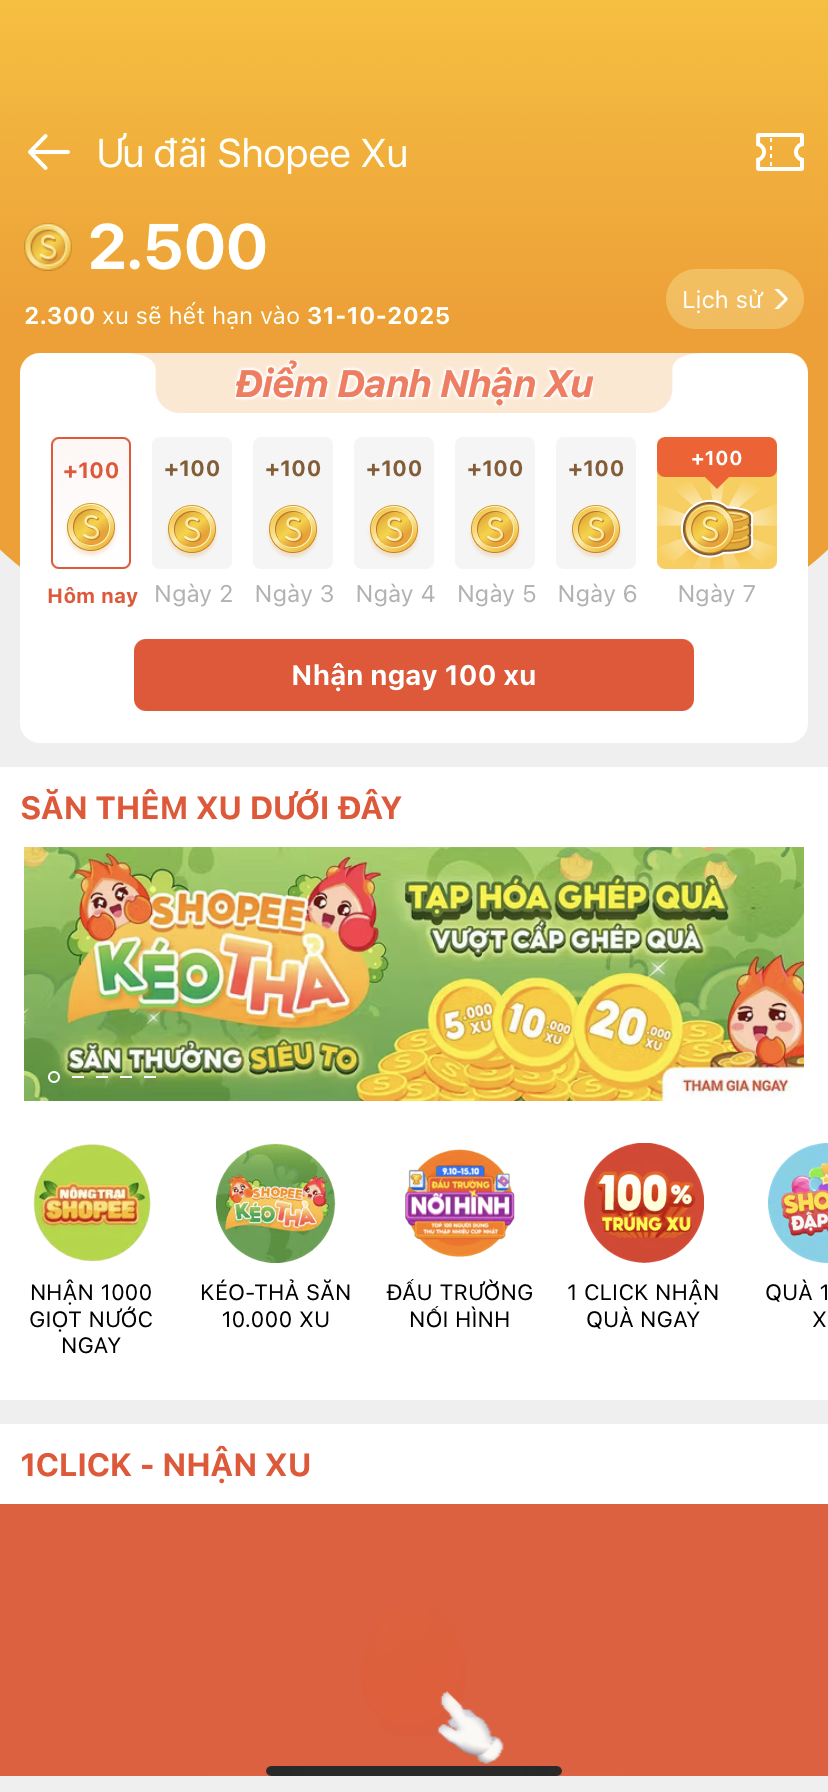
\includegraphics[width=0.6\textwidth]{Shopee_coins.PNG}
        \caption{Shopee xu của người dùng}
    \end{subfigure}
    \caption{Một số hình ảnh về hệ thống Shopee (tt)}
\end{figure}
% ảnh phần 4
\begin{figure}[H]
    \centering
    \begin{subfigure}[b]{0.4\textwidth}
        \centering
        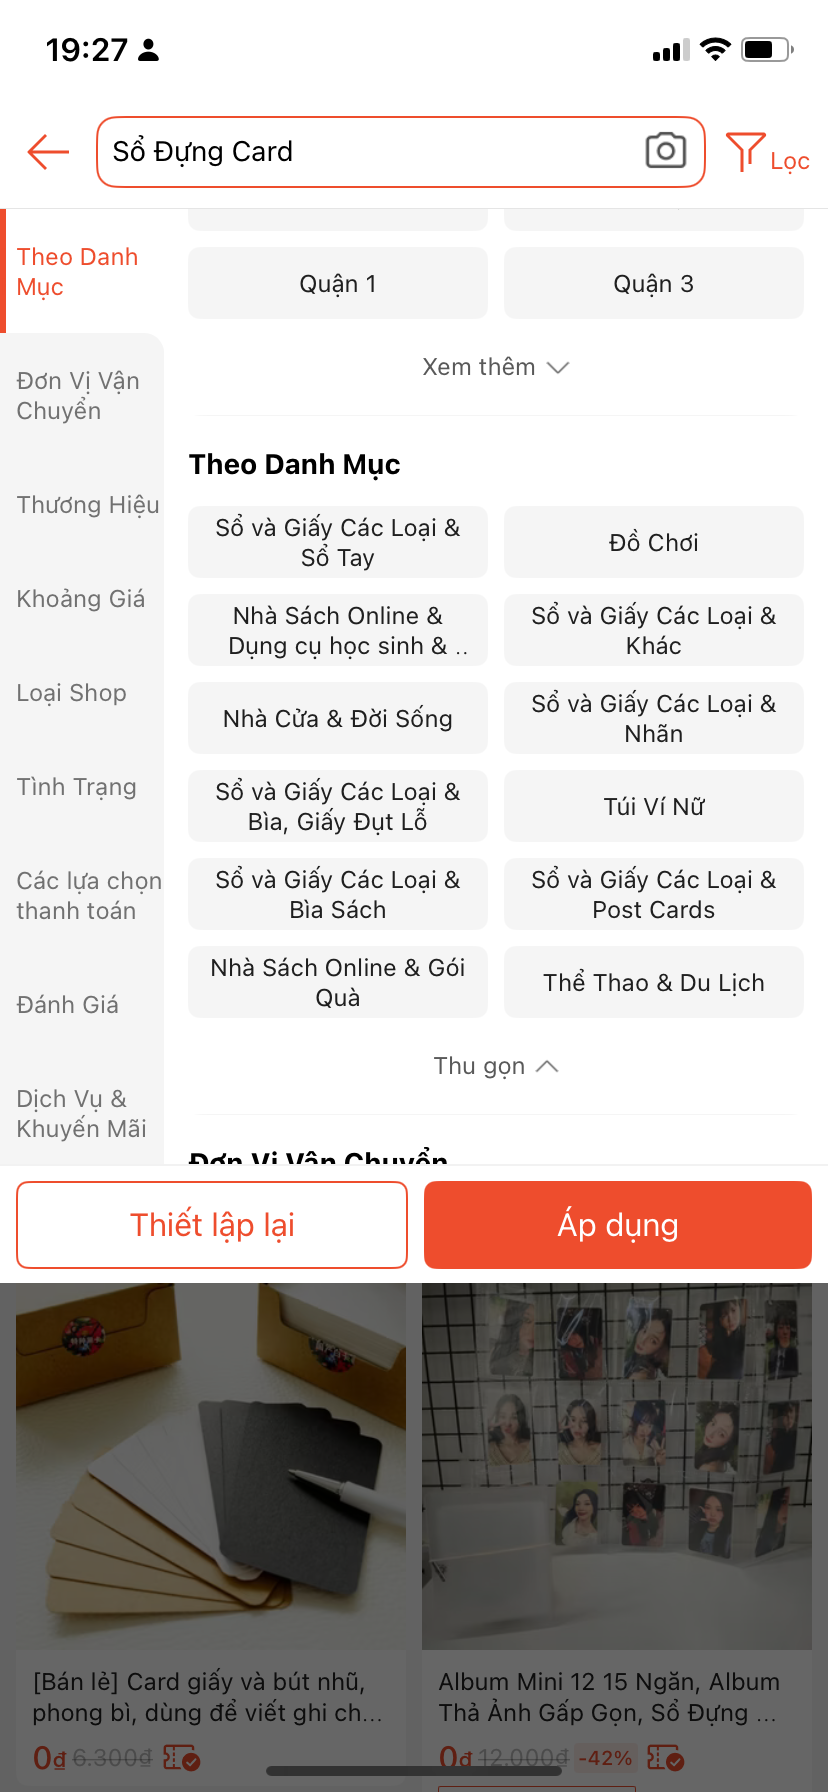
\includegraphics[width=0.6\textwidth]{Category.PNG}
        \caption{Danh mục của các sản phẩm}
    \end{subfigure}
    \hfill
    \begin{subfigure}[b]{0.4\textwidth}
        \centering
        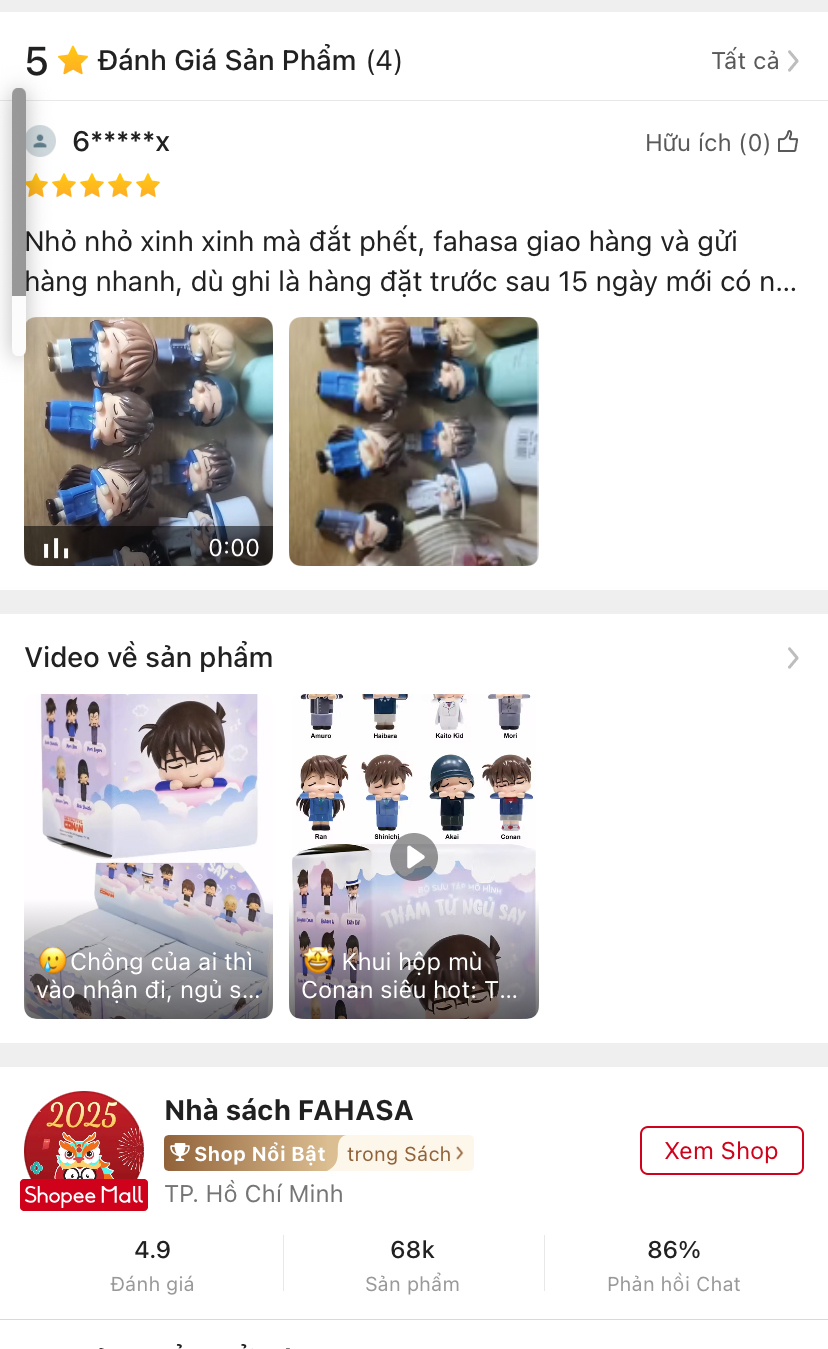
\includegraphics[width=0.6\textwidth]{Review_ratings.PNG}
        \caption{Đánh giá và rating của sản phẩm}
    \end{subfigure}
    \caption{Một số hình ảnh về hệ thống Shopee (tt)}
\end{figure}
% ảnh phần 5
\begin{figure}[H]
    \centering
    \begin{subfigure}[b]{0.4\textwidth}
        \centering
        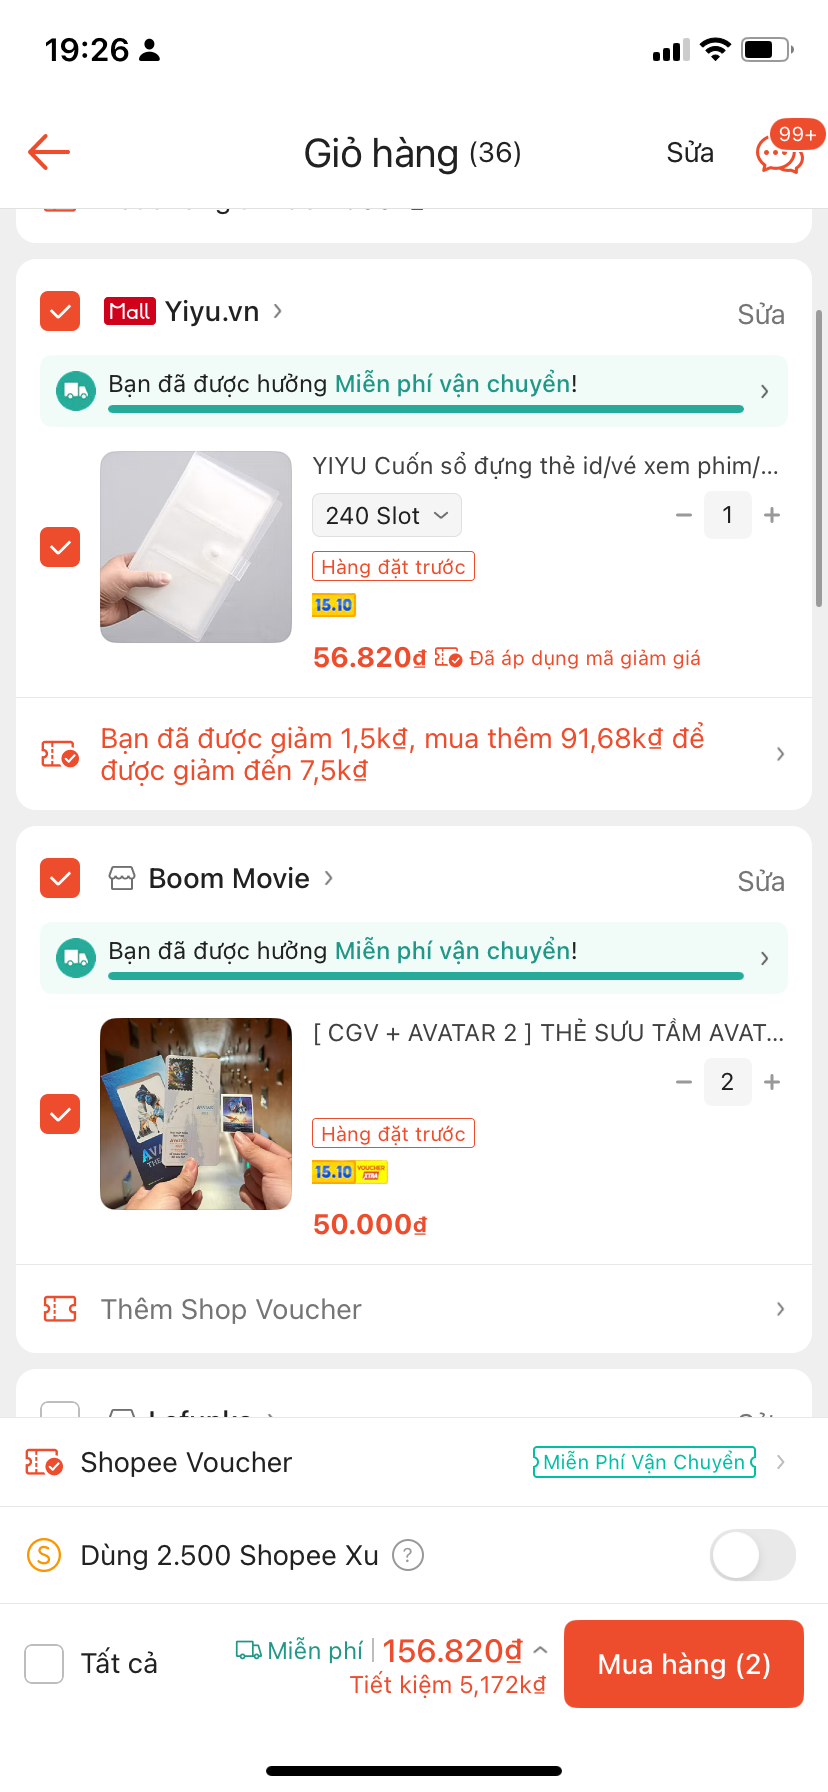
\includegraphics[width=0.6\textwidth]{Order_group.PNG}
        \caption{Nhóm đơn hàng khi đặt trong giỏ}
    \end{subfigure}
    \hfill
    \begin{subfigure}[b]{0.4\textwidth}
        \centering
        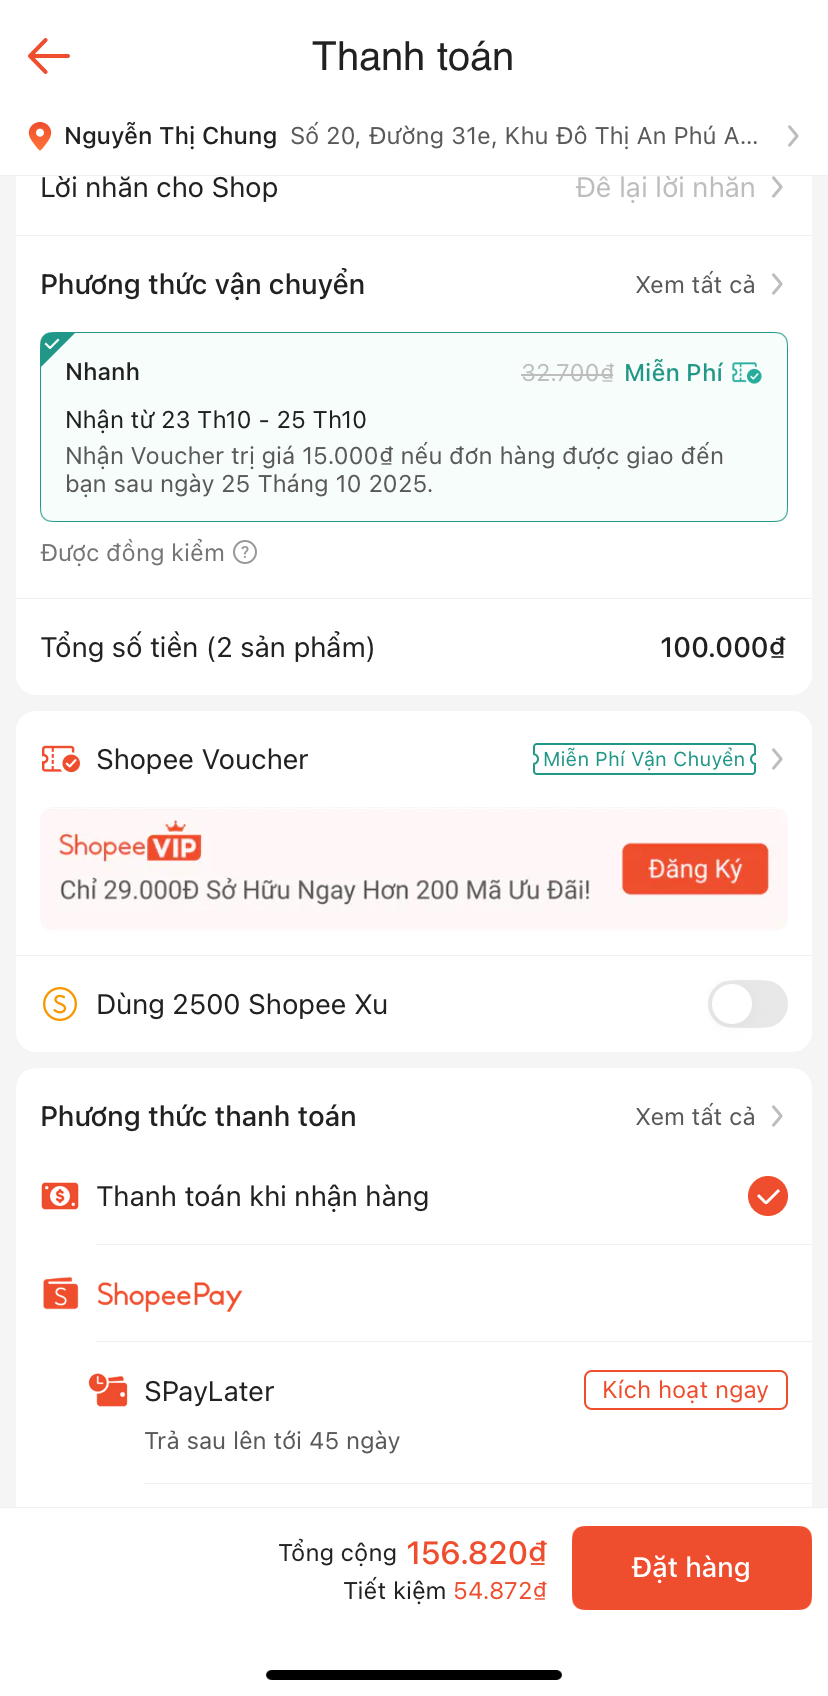
\includegraphics[width=0.6\textwidth]{Payment.PNG}
        \caption{Trang thanh toán}
    \end{subfigure}
    \caption{Một số hình ảnh về hệ thống Shopee (tt)}
\end{figure}
%ảnh cuối
\begin{figure}[H]
    \centering
    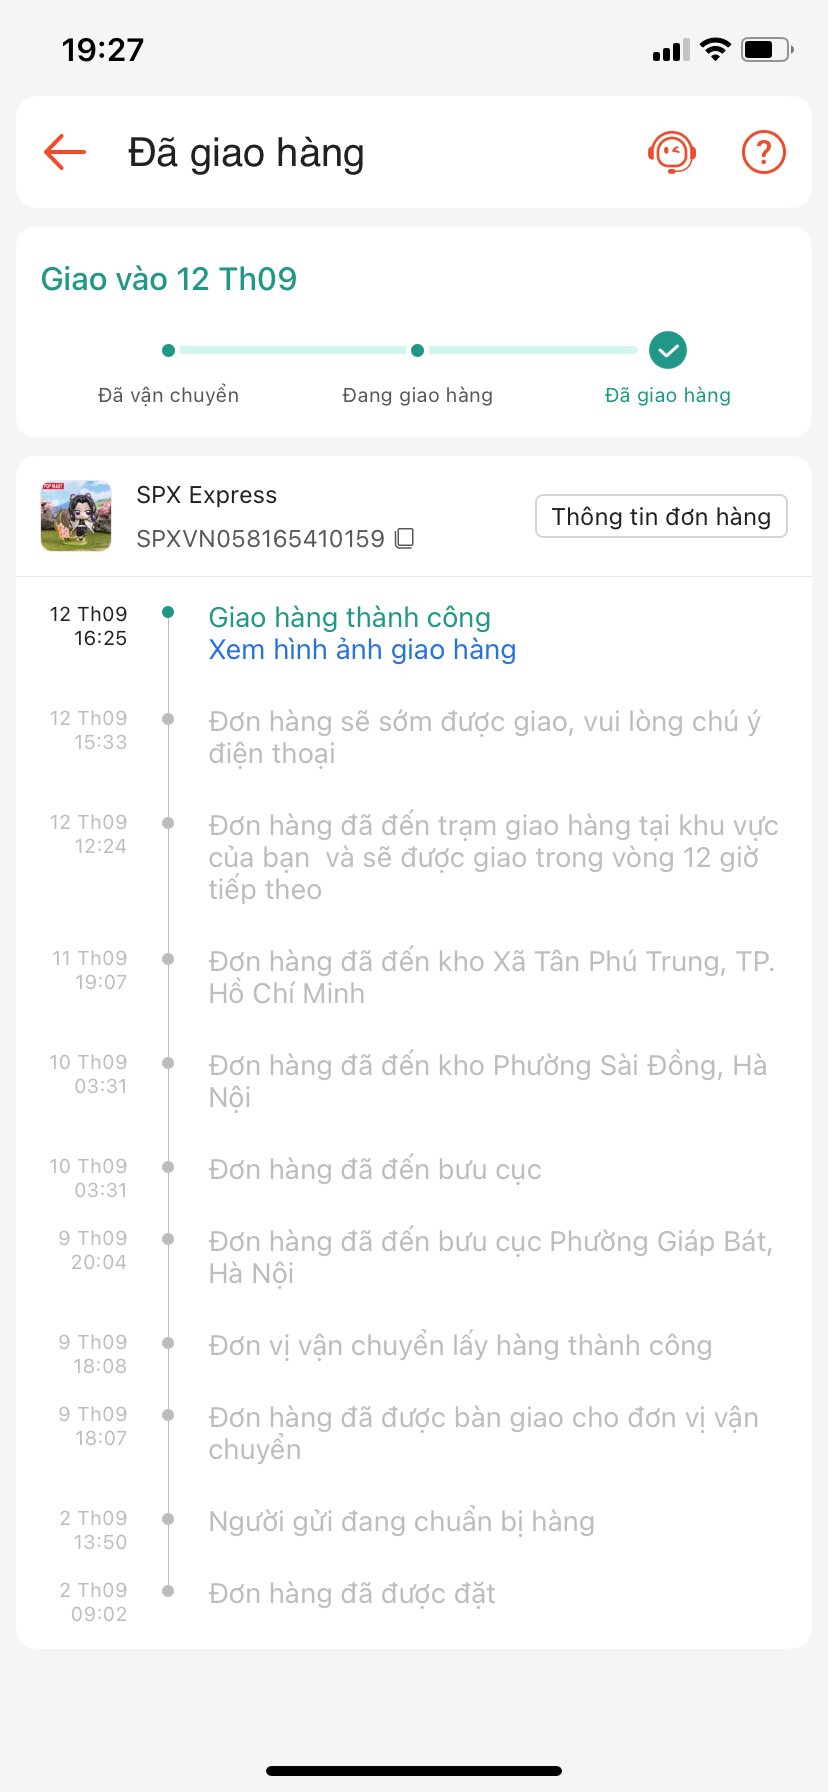
\includegraphics[width=0.4\textwidth]{Status.PNG}
    \caption{Tình trạng giao hàng}
\end{figure}
